\documentclass[11pt, a4paper]{article}
\usepackage[dutch, english]{babel}
\usepackage[pdftex]{graphicx}
\usepackage[linkcolor=black,urlcolor=blue,citecolor=black]{hyperref}
\usepackage[font=small,format=plain,labelfont=bf,up,textfont=it,up]{caption}
\usepackage[usenames,dvipsnames]{pstricks}
\usepackage{epsfig}
\usepackage[parfill]{parskip}
\hypersetup{colorlinks=true}
\usepackage{amsmath, epic, eepic, float, subfig, amsfonts, color, amsthm, textcomp, microtype, fullpage}
\usepackage[all]{xy}
\newcommand{\HRule}{\rule{\linewidth}{0.5mm}}
\DeclareMathOperator{\bgtan}{bgtan}

\usepackage{helvet}
\renewcommand*{\familydefault}{\sfdefault}

\begin{document}

\selectlanguage{dutch}
\begin{titlepage}
\begin{center}

\includegraphics[width=0.5\textwidth]{./logo.pdf}~\\[1cm]


\textsc{\Large Computerarchitectuur}\\[0.5cm]

\HRule \\[0.4cm]
{ \LARGE \bfseries Niet-grafische toepassingen voor GPU's}\\[0.4cm]
{\large \textit{ofwel \textbf{GPGPU}}}\\[0.2cm]

\HRule \\[1.5cm]

\begin{minipage}{0.4\textwidth}
\begin{flushleft} \large
\emph{Door:}\\
Haroen \textsc{Viaene}\\

\end{flushleft}
\end{minipage}
\begin{minipage}{0.4\textwidth}
\begin{flushright} \large
\large{1$^{\text{ste}}$ fase bachelor Elektronica-ICT}\\
\end{flushright}
\end{minipage}

\vfill

{\large 2014-2015}

\end{center}
\end{titlepage}

\newpage

\section*{Inhoud}

\tableofcontents

\newpage

\section{Inleiding}

Omdat onze grafische kaarten alsmaar groter worden, lijkt het logisch om nieuwe toepassingen te zoeken voor deze kaarten. Snel denk je al aan de ontdubbeling van de CPU, omdat die vaak onder grotere stress staat dan de GPU, maar dit is niet altijd zo haalbaar, omdat grafische kaarten niet vast op het moederbord zitten, maar in bijvoorbeeld een PCI-poort gestopt kunnen worden. CPU's echter moeten in een speciaal daarvoor gemaakte socket gestopt worden. Het is ook moeilijker voor de gemiddelde end-user om een CPU te vervangen. Daardoor zijn GPU's makkelijker up te graden. Het probleem is echter dat normaal gezien enkel videobewerkingen uitgevoerd worden in een GPU. GPGPU (het uitvoeren van standaard-taken op een GPU of General Processing on Graphics Processing Units) maakt gebruik van het grote aantal processen die tegelijk (maar op een lagere snelheid) in een GPU kunnen uitgevoerd worden. Een interessante manier om dit te vergelijken is om de CPU te zien als een team van 10 wetenschappers die snel heel moeilijke operaties kunnen uitvoeren. De GPU kan je dan vergelijken met een leger van 1000 man. Een individuele soldaat zal niet goed zijn in bijvoorbeeld het uitrekenen van een integraal. Maar als je de taak opdeelt in 1000 kleine optellingen, zullen ze waarschijnlijk zelfs sneller zijn dan de wetenschappers omdat ze met zo veel zijn. Bij GPGPU heb je dus nood aan heel specifiek opgedeelde taken, maar als je dat zo kan doen en het effici\"ent is om die berekening op te delen, zal dit een zeer grote versnelling opleveren, die makkelijk te vermeerderen is door het aantal GPU's te verhogen.\cite{gpgpu.org}

\newpage

\section{Wat is GPGPU?}

GPGPU, ofwel General-Purpose Computing on Graphics Processing Units is het uitvoeren van gewone rekenopdrachten op de grafische kaart. Als je aan GPGPU-computing wil doen, zal je dit waarschijnlijk in OpenCL doen (of Nvidia's CUDA). GPGPU is nog niet zo heel lang mogelijk omdat tot vanaf 2001 grafische kaarten nog niet zo heel geavanceerd waren. Dankzij het geavanceerder worden van videospelletjes, videobewerkingen, gecombineerd met het daardoor performanter worden van grafische kaarten maakte het haalbaar om deze ook te gebruiken voor andere taken.\cite{wikigpgpu}

\section{Opkomst van GPGPU}

In 2001 werd het mogelijk om floating-point- en shader-berekeningen uit te voeren op een GPU. Dit betekende de opkomst van GPGPU, omdat nu ook toepassingen die niet enkel gebruikt worden voor het tonen van beelden op een scherm, maar ook echte berekeningen mogelijk werden. Dit werd bewezen door het berekenen van matrixvermenigvuldigingen in 2001, dat voor het eerst sneller op een GPU uit te voeren was dan op een CPU. Na deze eerste toepassingen van GPGPU werden er frameworks zoals OpenGLen Microsoft's DirectX geschreven om gebruik van de vooruitgangen te kunnen maken in ander programma's. Later kwam NVidia met CUDA op de proppen, gevolgd door de meest recente Apple/Khronos OpenCL en Microsoft's DirectCompute. 

\section{Voordelen van GPGPU}

Omdat grafische kaarten van nature uit zich al parallel gedragen en grafische kaarten makkelijk verdubbelbaar zijn (door bijvoorbeeld twee grafische kaarten te installeren), zijn grafische kaarten een stuk flexibeler dan CPU's. Dit wil zeggen dat vooral bij lange berekeningen en dingen waar veel berekeningen tegelijk moeten gebeuren het zeer handig is om aan GPGPU te doen. In andere secties wordt er specifieker toegespitst op een aantal voorbeelden waarbij het handig is om die rekenopdrachten uit te voeren op grafische kaarten. Typische voorbeelden waarbij GPGPU handig is, zijn wiskundige berekeningen, cryptografie en ander wetenschappelijk onderzoek.

\section{Toepassingen van GPGPU}
\subsection{Wiskunde}

De eerste toepassingen van GPGPU waren matrixvermenigvuldigingen in 2001 en LU decompositie in 2005. Beide zijn bewerkingen op matrices. Matrices zijn van nature uit zeer ontdubbelbaar, omdat je altijd een hele hoop relatief simpele bewerkingen moet doen (optelling en vermenigvuldiging). Later zijn ook andere wiskundige toepassingen in de wiskunde gekomen. Ook AES- en RSA-encryptie lenen zich zeer goed tot het uitvoeren op grafische kaarten.

\subsection{Fysica}

Een aantal veelvoorkomende, maar toch zeer ingewikkelde problemen zijn onder andere het Ising-model\cite{ising} in de statistische fysica (waarmee ferromagnetisme gemodelleerd wordt), kwantumfysica, het berekenen van de beweging van onsamendrukbare vloeistoffen\cite{giancoli} met de Navier-Stokes-vergelijkingen, stroom van Newtoniaanse vloeistoffen (met de Lattice Boltzmann methode, die in plaats van de Navier-Stokes-vergelijkingen andere uitvoert, die gebruik maakt van een collisiestap en een vloeistap), de Monte Carlo methode\cite{montecarlo} (een methode die gebruikt wordt om dingen precies te schatten) etc.

\subsection{Biologie}

Biologische berekeningen die gebruik maken van GPGPU zijn meestal van bio-informatica-aard. Bio-informatica is de wetenschap van zowel het opmaken van programma's en methodes om biologische data te analyseren, als de wetenschap die deze data effectief analyseert. Qua GPGPU gaat het hier vooral over visalisuaties van genomen, chromosomen etc. Bij sequentie-analyse van DNA is het ook nuttig om de berekeningen op te splitsen en te laten uitvoeren door GPU's of GPU-clusters.

\begin{figure}[H]
	\centering
	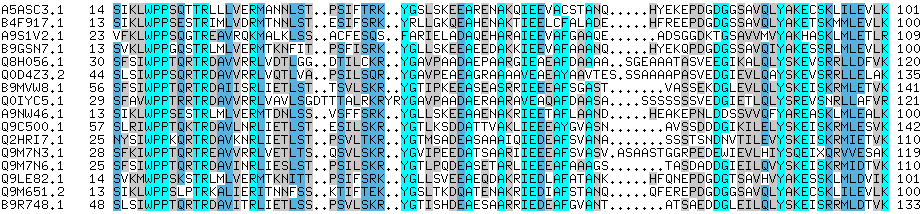
\includegraphics[width=\textwidth]{./bioinformatics.png}
	\caption{Het vergelijken van het genoom op het WPP-domein}	
\end{figure}

\subsection{Chemie}

Ook in de chemie is het haalbaar om zeer ingewikkelde berekeningen om te zetten in kleinere, meer haalbare berekeningen, die op grafische kaarten kunnen uitgevoerd worden. Dit gaat dan bijvoorbeeld over kwantumchemie. Ook het visualiseren van moleculen is een taak die effici\"ent is om op te delen in kleine subtaken die door GPU's kunnen worden uitgevoerd.

\subsection{Informatica}

Natuurlijk kunnen we binnen de informatica alles onderbrengen wat in de andere secties besproken wordt, maar specifiek voor de toepassingen van GPGPU in informatica wordt gedacht aan het opbouwen van high performance computerclusters (HPC clusters\cite{HPCClusters}), deze maken vaak gebruik van grafische kaarten omdat deze makkelijker ontdubbelbaar zijn. Bij MATLAB-servers wordt er vaak met verschillende GPU's gewerkt, omdat wiskundige taken als deze makkelijk opdeelbaar zijn.

\subsubsection{Cryptografie}

Cryptografie is het proces dat gebeurt bij het encrypteren van data. Dit gebeurt meestal met AES of RSA. Aan het einde van het vorige decennium werd het haalbaar om deze berekeningen op grafische kaarten uit te voeren. Bij cryptografie worden zeer veel ingewikkelde berekeningen tegelijk uitgevoerd. Dat maakt hiervan een goed voorbeeld om uit te voeren op grafische kaarten. 

Niet zo vaak geweten is dat de berekeningen die door cryptografische programma's uitgevoerd worden zo geproduceerd zijn dat ze te moeilijk zijn om met de middelen die op dat moment beschikbaar de encryptie te kraken.\cite{juniorcollege} Dit kraken houdt in dat je dezelfde berekeningen uitvoert op de uitgekomen getallen. Wat het nu echter zo moeilijk maakt om die berekeningen achterstevoor uit te voeren is dat wanneer je een priemfactorisatie moet maken van zeer grote getallen (dit is nodig om van een uitkomst aan de ingedutte waarden te raken), dat dit dagen, tot zelfs weken kan duren (afhankelijk van de graad van encryptie gebruikt en de hardware natuurlijk). 

\subsubsection{Cryptocurrencies} 

Cryptocurrencies zoals Bitcoin, Litecoin en Dogecoin maken gebruik van die cryptografie om een monetair systeem op te stellen. Virtuele munten zoals deze werken door middel van een zogenaamde blockchain. Alle geconfirmeerde transacties komen hierin terecht. Het stuk waarin cryptografie gebruikt wordt is het controleren van die transacties. In de beginperiode van die virtuele munten werden die op gewone GPU's uitgevoerd. GPU's zijn zeer handig voor het controleren van transacties (het zogenaamde \emph{minen}) omdat er daarvoor veel verschillende berekeningen tegelijk moeten gebeuren. In tegenstelling tot CPU's zijn GPU's zeer goed in parallelle berekeningen\cite{bitwiki}. Dit is het grote voordeel van GPGPU. Tegenwoordig worden die beperkingen echter op gespecialiseerde apparatuur gedaan zoals ASICMiner\cite{asicminer}, AntMiner\cite{antminer} en andere. Deze zijn zogenaamde ASIC's (circuits die voor een specifieke doeleinde gemaakt zijn)\cite{wikiasic}. \cite{bitcoin.org}


\subsection{Medische sector}

Bij bijvoorbeeld CT-scans en andere methodes van beeldverwerving is er nood aan snelle berekening van anomali\"en en een duidelijk beeld zodat er snel een diagnose kan gesteld worden. Hierbij is GPGPU handig, omdat die taken makkelijk onderverdeelbaar zijn in kleinere subtaken, die door een GPU kunnen worden uitgevoerd. Analyse van de uitspreiding van kanker is ook een proces waarop GPGPU toepasbaar is.

\section{conclusie}

Het kan dus zeer handig zijn om berekeningen uit te voeren op een grafische kaart, maar dit geldt enkel als de berekeningen of methodes opdeelbaar zijn, zodat je gebruik kan maken van de vele threads die een GPU heeft.

\newpage

\begin{thebibliography}{9}
	
\bibitem{gpgpu.org}
	\textbf{GPGPU}, 
	About GPGPU.org, 
	[geraadpleegd op 22 oktober 2014]. 
	\url{http://gpgpu.org/about}

\bibitem{wikigpgpu}
	\textbf{Wikipedia}, 
	General-purpose computing on graphics processing units, 
	[geraadpleegd op 22 oktober 2014]. 
	\url{http://en.wikipedia.org/wiki/General-purpose_computing_on_graphics_processing_units}.

\bibitem{ising}
	\textbf{Martin Weigel}, 
	Mini-Workshop “Simulations on GPU”, 
	Theoretische Physik, Universit\"at des Saarlandes, Saarbr\"ucken, Germany and Institut f\"ur Physik, Johannes-Gutenberg-Universit\"at Mainz, Germany

\bibitem{giancoli}
 	\textbf{Douglas C. Giancoli}, 
	Physics for Scientists \& Engineers with Modern Physics (6th Edition), 
	Pearson.

\bibitem{montecarlo}
	\textbf{Benjamin Block, Peter Virnau, Tobias Preis}, 
	Multi-GPU Accelerated Multi-Spin Monte Carlo Simulations of the 2D Ising Model, 
	Department of Physics, Mathematics and Computer Science, Johannes Gutenberg University Mainz 
	
\bibitem{HPCClusters}
	\textbf{Volodymyr V. Kindratenko, Jeremy J. Enos, Guochun Shi, Michael T. Showerman, Galen W. Arnold, John E. Stone, James C. Phillips, Wen-mei Hwu}, 
	GPU Clusters for High-Performance Computing, 
	University of Illinois at Urbana-Champaign. 

\bibitem{juniorcollege}
	\textbf{Junior College 2012-2013}, 
	van priemgetal tot digitale handtekening, 
	KU Leuven faculteit Wetenschap \& Technologie.
	
\bibitem{wikiasic}
	\textbf{Wikipedia}, 
	Application-specific integrated circuit. 
	[geraadpleegd op 27 oktober 2014]. 
	\url{http://en.wikipedia.org/wiki/Application-specific_integrated_circuit}
	
\bibitem{bitwiki}
	\textbf{Bitcoin Wiki}, 
	Why a GPU mines faster than a CPU. 
	[geraadpleegd op 23 oktober 2014]. 
	\url{https://en.bitcoin.it/wiki/Why_a_GPU_mines_faster_than_a_CPU}

\bibitem{asicminer}
	\textbf{Bitcointalk}, 
	ASICMiner Publicly Looking for Potential Customers/Partners for New Chips,  
	[geraadpleegd op 27 oktober 2014]. 
	\url{https://bitcointalk.org/index.php?topic=438359.0}

\bibitem{antminer}
	\textbf{Bitmain}, 
	Products. 
	[geraadpleegd op 27 oktober 2014]. 
	\url{https://www.bitmaintech.com/product.htm}	

\bibitem{bitcoin.org}
	\textbf{Bitcoin}, 
	How does Bitcoin work? 
	[geraadpleegd op 27 oktober 2014]. 
	\url{https://bitcoin.org/en/how-it-works}
\end{thebibliography}

\end{document}  